

Logs are leveraged by developers to record useful information during the execution of an application. Logs are recorded during various development activities such as bug fixing~\cite{ConsoleLogs,JGLouMining,QFuanomaly}, load test analysis~\cite{Automatic}, monitoring performance~\cite{Yuan} and for knowledge transfer~\cite{IanWCRE}.
Logging can be done through the use of log libraries or more archaic methods such as \textsl{print} statements. Every log\footnote{
In the rest of this paper, we use ‘log’ to refer to the logging statements in the source code.} contains a textual part, which provides information about the context, a variable part providing context information about the event and a log level, which shows the verbosity of the logs. An example of a log is shown below where info is the logging level, \textsl{Testing Connection to Host Id} is the context information and \textsl{host}, which is the variable part, provides information about the logging context.
\hypobox{LOG.info(``Testing Connection to Host Id:" + host);}

\begin{figure}[tb]
	\centering
	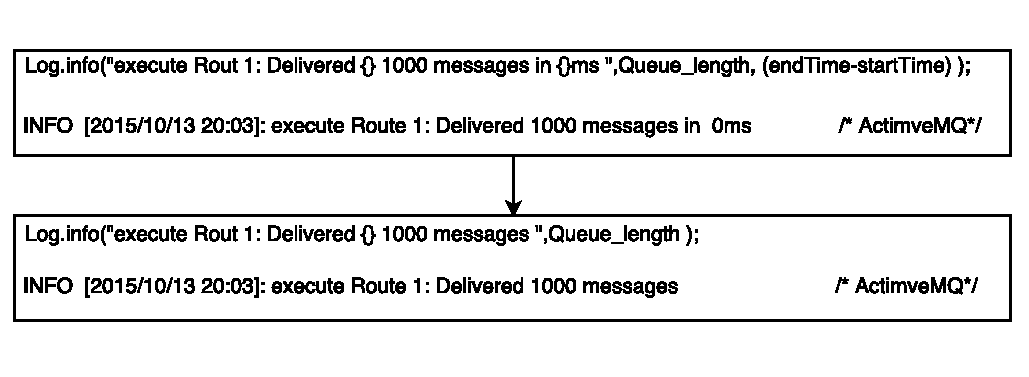
\includegraphics[width=1\columnwidth]{ExampleOfLogChange_LPA}
	\caption{Modification of a logging statement}
	\label{fig:ExampleOfLogChange_LPA}
\end{figure}


The rich knowledge in logs has lead to the development of many enterprise log processing tools such as \textsl{Splunk}~\cite{carasso2012exploring}, \textsl{Xpolog}~\cite{xpolog}, \textsl{Logstash}~\cite{xu2013detecting} and research tools such as Salsa~\cite{TanSalsa}, log-enhancer~\cite{Yuan} and Chukwa~\cite{chukwa} which are designed to analyze as well as improve logs in software applications. However, when logs are changed, the associated log processing tools may also need to be updated. For example, Figure~\ref{fig:ExampleOfLogChange_LPA} demonstrates a case in which a developer removes the time taken for completing an event. This can affect log processing tools that rely on the removed information in-order to monitor the health of the application. Prior research shows that 60\% of the logs which are output during system execution are changed and affect the log processing tools that heavily depend on such logs~\cite{IanWCRE}.

% These log changes can affect the log processing tools which heavily depend on them and maintenance cost will be high~\cite{IanWCRE}. 

\begin{figure*}
	\centering
	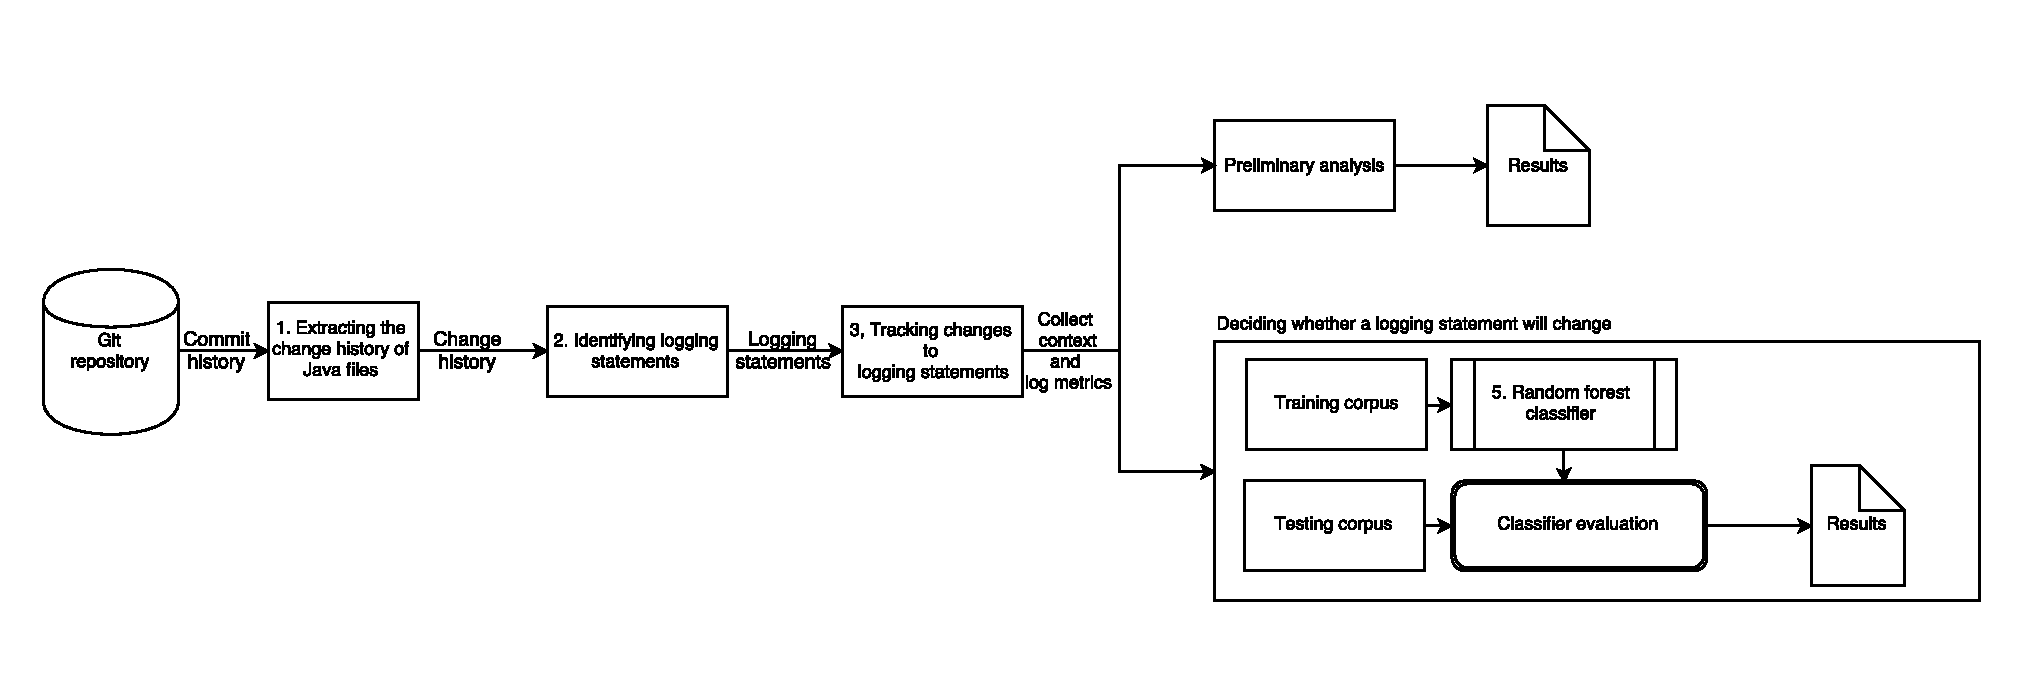
\includegraphics[width=1\textwidth,
	height=.4\textwidth]{LogGenalogyMethdology}
	\caption{Overview of the data extraction and case study approach}
	\label{fig:LGmethod}
\end{figure*}


In this paper, we study the changes that are made to logs across multiple releases in four studied open source applications. We find that 35\%-50\% of the logs are changed at least once during their lifespan in the studied applications. We find that a single log changes between 1 to 12 times within its lifetime and can be changed by more than one developer. To identify which factors play a vital role in the stability of logging statements and model which logs will change in future, we build a random forest classifier using context and log metrics. The most important observations in this paper are:
\begin{enumerate}
	\item  Our \textsl{random forest} achieves an precision of 89\%-91\% and recall of 71\%-83\%, when predicting which logs will be changed.
	\item Logs introduced in a file by developers who have less ownership of that file are more likely to be changed later than logs written by owners of the file. 
	\item Files with a higher log density are less likely to have changes made to their logs than files with a lower log density.
	\item Developer experience is negatively correlated to log stability in the studied applications, suggesting that logs introduced by more experienced developers are more stable. 
%	\item  Change metrics such as SLOC, number of variables logged and number of variables declared are strong predictors of log stability within the studied applications. 

\end{enumerate}



%These log processing tools are used to generate information for capacity planning of large-scale systems~\cite{hassan2008industrial,nagappan2009efficiently}, to monitor system health~\cite{bitincka2010optimizing} or to detect abnormal system behavior~\cite{JiangICSM2008}. These tools rely heavily on the log messages themselves and require continuous maintenance when the format or content of logs are changed.

% and use the data to answer the following research questions.

%\textbf{RQ1:} \textbf{How much do logs change over time and why do the changes occur?}
%
%Based on our quantitative analysis of the studied systems we identify three categories of change frequency in logs. If a log is changed more than four times we categorize it as \textsl{`Frequently Changed'}, if it has one to three changes, it is categorized as \textsl{`Changed'} and if there are no changes made we categorize it as \textsl{`Never Changed'}. We find that in our studied systems, 20-80\% of the logs are changed at least once throughout their lifespan.


%\textbf{RQ2:} \textbf{Can metrics from code, log and developer dimension help in explaining the stability of logs?}

%We collect the product and change metrics from three dimensions namely code, log and developer information. Our \textsl{random forest} achieves an accuracy of 89\%-91\% and recall of 71\%-91\%, when predicting which logs have higher likelihood of getting changed. We also identify significant metrics from each of the three dimensions, that affect the stability of logs. We find  developer experience, source lines of code, file ownership, log density in the file are strong predictors in classifying if a log will change in the future. 
 
 
% Our results show that product and process metrics obtained from code, log and developer information can help in identifying unstable logs in our studied systems. This can help in reducing the effort needed in the maintenance of log processing applications, as system maintainers can flag the logs that have the potential of being changed in subsequent releases and track them. 
 
The remainder of this paper is organized as follows. Section~\ref{analysis} presents the preliminary analysis to motivate our study. Section~\ref{prediction} describes the random forest classifier and the analysis results. Section~\ref{related} describes the prior research that is related to our work. Section~\ref{threats} discusses the threats to validity. Finally, Section~\ref{conc} concludes the paper.
 
 
% However, as these tools are not scalable for all companies and systems, companies prefer in house development or customization of these tools for their specific purposes. 